\documentclass[pdftex,12pt,xcolor=svgnames]{beamer}

\mode<presentation>
{
  \usetheme{boxes}
  \usecolortheme[named=MidnightBlue]{structure}
  %\setbeamercolor{normal text}{bg=NavajoWhite!20}
  \usefonttheme{serif}
  \setbeamertemplate{navigation symbols}{}
  % Show frame number and author name in footline
  \setbeamertemplate{footline}[frame number]
  \addtobeamertemplate{footline}{\quad\textcolor{gray}{David Duvenaud}}{}
  % Set frame titles in small capitals
%  \setbeamerfont{frametitle}{shape=\scshape,family=\rmfamily}
  \setbeamerfont{frametitle}{family=\rmfamily}
  \setbeamercolor{frametitle}{bg=gray!10!white,fg=black}
  % Alerted text: blue (uncomment second line if theme sets alerted text to bold)
  \setbeamercolor{alerted text}{fg=blue}
  %\setbeamerfont*{alerted text}{}
  \setbeamertemplate{bibliography item}[text] %{\hbox{\donotcoloroutermaths$\blacktriangleright$}}
  \setbeamertemplate{bibliography entry title}{}
  \setbeamertemplate{bibliography entry author}{}
  \setbeamertemplate{bibliography entry note}{}
  \setbeamertemplate{bibliography entry location}{}

}
\usepackage[english]{babel}
\usepackage[latin1]{inputenc}
\usepackage{times}
\usepackage[T1]{fontenc}
\usepackage{hyperref}
\usepackage{multimedia}
\usepackage{eepic}
\usepackage{graphicx}
%\usepackage[nohug]{latexinclude/diagrams}
\usepackage{tikz}
\usetikzlibrary{calc}

%% \newcommand{\footlineextra}[1]{
%%     \begin{tikzpicture}[remember picture,overlay]
%%         \node[yshift=1.5ex,anchor=south east] at (current page.south east)
%% {#1};
%%     \end{tikzpicture}
%% }

\newcommand{\footlineextra}[1]{
    \begin{tikzpicture}[remember picture,overlay]
        \node[xshift=-5ex,yshift=-0.5ex,anchor=south east] at (current page.south east)
             {\mbox{\tiny \textcolor{MidnightBlue}{#1}}};
    \end{tikzpicture}
}

\def\sectionframe#1{
  {
    \setbeamertemplate{footline}{\empty}
    \begin{frame}{}
      \begin{center}
%        \huge\sc #1
	\huge #1
      \end{center}
    \end{frame}
  }
}


\usepackage{etex}
%% This file provides examples of some useful macros for typesetting
% dissertations.  None of the macros defined here are necessary beyond
% for the template documentation, so feel free to change, remove, and add
% your own definitions.
%
% We recommend that you define macros to separate the semantics
% of the things you write from how they are presented.  For example,
% you'll see definitions below for a macro \file{}: by using
% \file{} consistently in the text, we can change how filenames
% are typeset simply by changing the definition of \file{} in
% this file.
% 
%% The following is a directive for TeXShop to indicate the main file
%%!TEX root = diss.tex

\newcommand{\pd}{\mbox{pd}}
\newcommand{\tr}{\mbox{tr}}
\newcommand{\mbf}[1]{\mbox{\boldmath $#1$}}
\newcommand{\deriv}[2]{\frac{\partial #1}{\partial #2}}
\newcommand{\mean}{\mathop{\mbox{mean}}}
\newcommand{\median}{\mathop{\mbox{median}}}
\newcommand{\diag}{\mbox{diag}}
\newcommand{\trace}{\mbox{trace}}
\newcommand{\st}{\mbox{st}}
\newcommand{\FF}{\tilde{F}}
\newcommand{\cut}[1]{}
\newcommand{\vn}{\varnothing}
\def\argmax{\operatornamewithlimits{arg\,max}}
\def\argmin{\operatornamewithlimits{arg\,min}}
\def\theequation{\arabic{section}.\arabic{equation}}
\def\thedefinition{\arabic{section}.\arabic{definition}}
\def\thetheorem{\arabic{section}.\arabic{theorem}}
\def\theexample{\arabic{section}.\arabic{example}}

\newcommand{\NA}{\textsc{n/a}}	% for "not applicable"
\newcommand{\eg}{e.g.,\ }	% proper form of examples (\eg a, b, c)
\newcommand{\ie}{i.e.,\ }	% proper form for that is (\ie a, b, c)
\newcommand{\etal}{\emph{et al}}

\newcommand{\expect}{\mathbb{E}}
\newcommand{\variance}{\mathbb{V}}
\newcommand{\bx}{{\bf x}}
\newcommand{\by}{{\bf y}}
\newcommand{\bX}{{\bf X}}
\newcommand{\bK}{{\bf K}}
\newcommand{\bs}{{\bf s}}
\newcommand{\bu}{{\bf u}}
\newcommand{\bff}{{\bf f}}

%\documentclass[usenames,dvipsnames]{beamer}
%\usepackage{beamerthemesplit}
%\usepackage{graphics}
%\usepackage{amsmath}
%\usepackage{rotating}
%\usepackage{array}
%\usepackage{nth}
\usepackage{xcolor}
\usepackage{textcomp}
\usepackage{listings}
%\usepackage[usenames,dvipsnames]{color}
% This is the color used for MATLAB comments below
\definecolor{MatlabDarkGreen}{rgb}{0.0,0.4,0.0}
\definecolor{Blue}{rgb}{0.0,0.0,1.0}

% For faster processing, load Matlab syntax for listings
\lstloadlanguages{Matlab}%
\lstset{language=Matlab,                        % Use MATLAB
        frame=single,                           % Single frame around code
        basicstyle=\tiny\ttfamily,             % Use small true type font
        keywordstyle=[1]\color{Blue}\bf,        % MATLAB functions bold and blue
        keywordstyle=[2]\color{Purple},         % MATLAB function arguments purple
        keywordstyle=[3]\color{Blue}\underbar,  % User functions underlined and blue
        identifierstyle=,                       % Nothing special about identifiers
                                                % Comments small dark green courier
        commentstyle=\usefont{T1}{pcr}{m}{sl}\color{MatlabDarkGreen}\tiny,
        stringstyle=\color{Purple},             % Strings are purple
        showstringspaces=false,                 % Don't put marks in string spaces
        tabsize=5,                              % 5 spaces per tab
        %
        %%% Put standard MATLAB functions not included in the default
        %%% language here
        morekeywords={xlim,ylim,var,alpha,factorial,poissrnd,normpdf,normcdf},
        %
        %%% Put MATLAB function parameters here
        morekeywords=[2]{on, off, interp},
        %
        %%% Put user defined functions here
        morekeywords=[3]{FindESS, homework_example},
        %
        morecomment=[l][\color{Blue}]{...},     % Line continuation (...) like blue comment
        numbers=left,                           % Line numbers on left
        firstnumber=1,                          % Line numbers start with line 1
        numberstyle=\tiny\color{Blue},          % Line numbers are blue
        stepnumber=50                            % Line numbers go in steps of 5
        }

% Includes a MATLAB script.
% The first parameter is the label, which also is the name of the script
%   without the .m.
% The second parameter is the optional caption.
\newcommand{\matlabscript}[2]
  {\begin{itemize}\item[]\lstinputlisting[caption=#2,label=#1]{#1.m}\end{itemize}}


\usepackage{tabularx}
\usepackage{picins}
\usepackage{tikz}
\usepackage{changepage}
\usepackage{wasysym} % for smileys

\usetikzlibrary{shapes.geometric,arrows,chains,matrix,positioning,scopes,calc}
\tikzstyle{mybox} = [draw=white, rectangle]

\definecolor{camlightblue}{rgb}{0.601 , 0.8, 1}
\definecolor{camdarkblue}{rgb}{0, 0.203, 0.402}
\definecolor{camred}{rgb}{1, 0.203, 0}
\definecolor{camyellow}{rgb}{1, 0.8, 0}
\definecolor{lightblue}{rgb}{0, 0, 0.80}
\definecolor{white}{rgb}{1, 1, 1}
\definecolor{whiteblue}{rgb}{0.80, 0.80, 1}
\definecolor{mydarkblue}{rgb}{0.00,0.08,0.45}

\newcolumntype{x}[1]{>{\centering\arraybackslash\hspace{0pt}}m{#1}}
\newcommand{\tabbox}[1]{#1}

% Deep net notation
\def\onefeat{h}
\def\feat{\vh}
\newcommand{\netweights}{w}
\newcommand{\vnetweights}{\vw}
\newcommand{\mnetweights}{\vW}


%%%%%%%%%%%%%%%%%%%%%%%%%%%%%%%%%%%%%%%%%%%
%
% Some look and feel definitions
%
%%%%%%%%%%%%%%%%%%%%%%%%%%%%%%%%%%%%%%%%%%%

\setlength{\columnsep}{0.03\textwidth}
\setlength{\columnseprule}{0.0018\textwidth}
\setlength{\parindent}{0.0cm}

%% This file provides examples of some useful macros for typesetting
% dissertations.  None of the macros defined here are necessary beyond
% for the template documentation, so feel free to change, remove, and add
% your own definitions.
%
% We recommend that you define macros to separate the semantics
% of the things you write from how they are presented.  For example,
% you'll see definitions below for a macro \file{}: by using
% \file{} consistently in the text, we can change how filenames
% are typeset simply by changing the definition of \file{} in
% this file.
% 
%% The following is a directive for TeXShop to indicate the main file
%%!TEX root = diss.tex

\newcommand{\pd}{\mbox{pd}}
\newcommand{\tr}{\mbox{tr}}
\newcommand{\mbf}[1]{\mbox{\boldmath $#1$}}
\newcommand{\deriv}[2]{\frac{\partial #1}{\partial #2}}
\newcommand{\mean}{\mathop{\mbox{mean}}}
\newcommand{\median}{\mathop{\mbox{median}}}
\newcommand{\diag}{\mbox{diag}}
\newcommand{\trace}{\mbox{trace}}
\newcommand{\st}{\mbox{st}}
\newcommand{\FF}{\tilde{F}}
\newcommand{\cut}[1]{}
\newcommand{\vn}{\varnothing}
\def\argmax{\operatornamewithlimits{arg\,max}}
\def\argmin{\operatornamewithlimits{arg\,min}}
\def\theequation{\arabic{section}.\arabic{equation}}
\def\thedefinition{\arabic{section}.\arabic{definition}}
\def\thetheorem{\arabic{section}.\arabic{theorem}}
\def\theexample{\arabic{section}.\arabic{example}}

\newcommand{\NA}{\textsc{n/a}}	% for "not applicable"
\newcommand{\eg}{e.g.,\ }	% proper form of examples (\eg a, b, c)
\newcommand{\ie}{i.e.,\ }	% proper form for that is (\ie a, b, c)
\newcommand{\etal}{\emph{et al}}

\newcommand{\expect}{\mathbb{E}}
\newcommand{\variance}{\mathbb{V}}
\newcommand{\bx}{{\bf x}}
\newcommand{\by}{{\bf y}}
\newcommand{\bX}{{\bf X}}
\newcommand{\bK}{{\bf K}}
\newcommand{\bs}{{\bf s}}
\newcommand{\bu}{{\bf u}}
\newcommand{\bff}{{\bf f}}

\usepackage{preamble}
\hypersetup{colorlinks=true,citecolor=blue}
%\pdfmapfile{+sansmathaccent.map}

\title{Visualizing Priors on Deep Functions}


\author{
\hspace{-1cm}
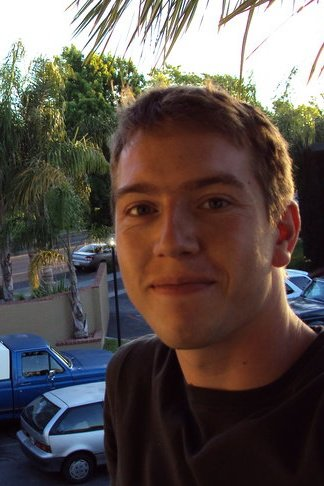
\includegraphics[height=0.2\textwidth, trim=20mm 25mm 0mm 25mm, clip]{figures/david2}
\qquad\quad
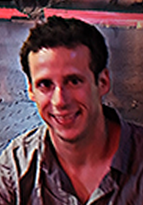
\includegraphics[height=0.2\textwidth]{figures/rippel2}
\qquad\quad
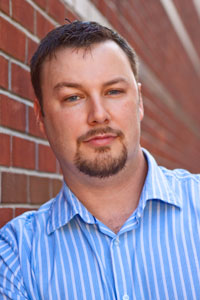
\includegraphics[height=0.2\textwidth]{figures/adams}
\qquad\quad
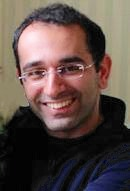
\includegraphics[height=0.2\textwidth]{figures/zg2}
\hspace{-1cm}
\\
\hspace{-0.9cm}
David Duvenaud, Oren Rippel, Ryan Adams, Zoubin Ghahramani
\hspace{-0.9cm}
}

\institute{
%\includegraphics[width=0.4\textwidth]{figures/spiral_main}
}
%\date{}


\begin{document}

%\setbeamertemplate{background canvas}{\begin{tikzpicture}\node[opacity=.1]{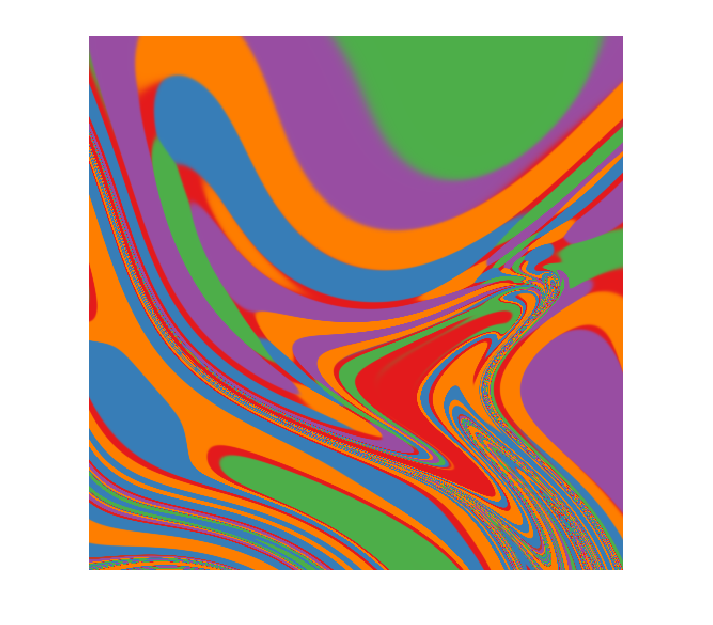
\includegraphics [width=\paperwidth]{figures/map_connected/latent_coord_map_layer_40}};\end{tikzpicture}}
\setbeamertemplate{background canvas}{\centering 
\begin{tikzpicture}\node[opacity=.2]{\centering 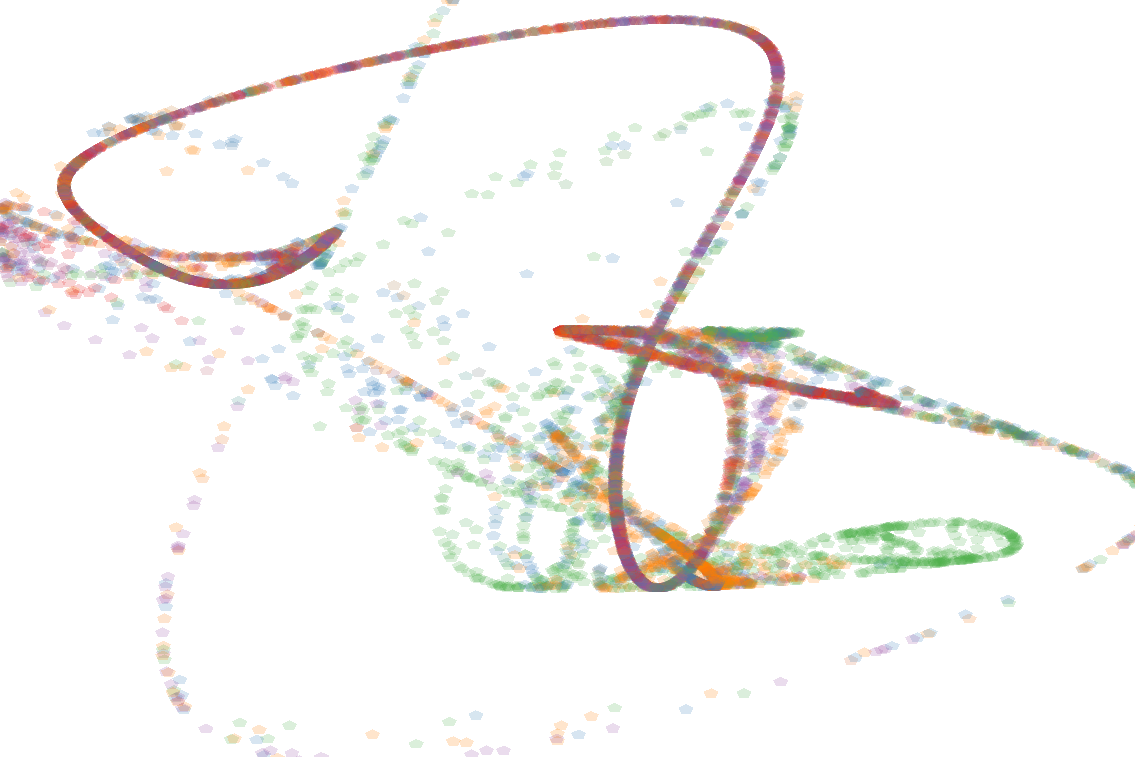
\includegraphics [width=\paperwidth]{figures/deep_gp_movie_486}};\end{tikzpicture}}



\frame[plain] {
\titlepage
}

\setbeamertemplate{background canvas}{}



\frame[plain]{
\frametitle{Motivation 1: Deep nets are hard to characterize}
\begin{itemize}
%	\item Don't you wish we were doing it?
%	\item Zoubin (2011) ``Do you guys ever wonder if this lab focuses too much on Gaussian processes?  Like maybe we're going to miss the next big thing, like maybe, say, deep learning''
	\item deep learning experiments are annoying, too many fiddly parameters
	\item But - GPs are just neural nets, we can make them deep!
\end{itemize}
}

\frame[plain]{
\frametitle{Motivation 2: Large nets are hard to regularize}
\begin{itemize}
	\item Neural nets are getting larger
	\item How to regularize billions of parameters?
	\item Closely related to constructing priors
	\item Priors are easy to analyze - just sample from the prior and look and what sorts of things you get!
%	\item \color{blue} Can we write a useful paper without doing any experiments?
	\item \color{blue} Can we suggest new regularization schemes or network architectures?
\end{itemize}
}



%\frame[plain]{
%\frametitle{Outline}
%\begin{itemize}
%	\item Relation between GPs and neural nets
%	\item Two ways to deepness:
%	\begin{itemize}
%		\item Deep kernels
%		\item Deep GPs
%	\end{itemize}
%	\item What kind of prior on functions do we want?
%	\begin{itemize}
%		\item problems with lots of indepenent layers
%		\item a simple fix
%	\end{itemize}
%	\item Dropout for GPs
%	\begin{itemize}
%		\item Dropping out features
%		\item Dropping out inputs
%	\end{itemize}	
%\end{itemize}
%}


\newsavebox\unistrain
\begin{lrbox}{\unistrain}
\hspace{0.1cm}
  \begin{minipage}{0.53\textwidth}
A weighted sum of features,
    \begin{align*}
%\feat(\vx) & = \vh^{(1)}(\vx) = \sigma \left( \vb^{(1)} + \vW^{(1)}\vx \right) \\
%f(\vx) & = \vV^{(1)} \sigma \left( \vb^{(1)} + \vW^{(1)} \vh^{(1)}(\vx) \right)  = \vV^{(1)} \vh^{(1)}(\vx) \\
f(\vx) & %= \frac{1}{K}{\mathbf \netweights}\tra \feat(\vx) 
= \frac{1}{K} \sum_{i=1}^K \netweights_i \onefeat_i(\vx)
    \end{align*} 
with any weight distribution,
    \begin{align*}
%\feat(\vx) & = \left[ \onefeat_1(\vx), \dots, \onefeat_K(\vx) \right]\tra \\
\expectargs{}{\netweights_i} & = 0, \quad \varianceargs{}{\netweights_i} = \sigma^2, \quad \iid
    \end{align*} 
by CLT, gives a GP as $K \to \infty$!
        \begin{align*}
%\lim_{K \to \infty} & \left[ f(\vx), f(\vx') \right ]\tra 
\cov \left[ \! \begin{array}{c} f(\vx) \\ f(\vx') \end{array} \! \right] \to \frac{\sigma^2}{K}\sum_{i=1}^K \onefeat_i(\vx)\onefeat_i(\vx')
    \end{align*} 
  \end{minipage}
\end{lrbox}


\def\layersep{2cm}
\def\nodesep{1.5cm}
\def\nodesize{1cm}

\newcommand{\numdims}[0]{3}
\newcommand{\numouts}[0]{1}
\newcommand{\numhidden}[0]{4}
\newcommand{\upnodedist}[0]{1cm}
\newcommand{\bardist}[0]{\hspace{-0.2cm}}

\frame[plain]{
\frametitle{GPs as Neural Nets}

\vspace{0.5cm}
\begin{tabular}{c|c}
\hspace{-1.25cm}
\begin{minipage}{0.54\textwidth}
\begin{tikzpicture}[shorten >=1pt,->,draw=black!50, node distance=\layersep]
    \tikzstyle{every pin edge}=[<-,shorten <=1pt]
    \tikzstyle{neuron}=[circle,fill=black!25,minimum size=17pt,inner sep=0pt]
    \tikzstyle{input neuron}=[neuron, fill=green!30];
    \tikzstyle{output neuron}=[neuron, fill=red!30];
    \tikzstyle{hidden neuron}=[neuron, fill=blue!30];
    \tikzstyle{annot} = [text width=4em, text centered]

    % Draw the input layer nodes
    \foreach \name / \y in {1,...,\numdims}
    % This is the same as writing \foreach \name / \y in {1/1,2/2,3/3,4/4}
        \node[input neuron, minimum size=\nodesize
        %, pin=left:Input \#\y
        ] (I-\name) at (0,-\nodesep*\y) {$x_\y$};

    % Draw the hidden layer nodes
    \foreach \name / \y in {1,...,\numhidden}
        \path[yshift=0.5cm]
            node[hidden neuron, minimum size=\nodesize] (H-\name) at (\layersep,-\nodesep*\y) {$\onefeat_\y(\vx)$};

    % Draw the output layer node
    \foreach \name / \y in {1,...,\numouts}
    	\node[output neuron, minimum size=\nodesize
    	%,pin={[pin edge={->}]right:Output }
    	] (O-\name) at (2*\layersep,-\nodesep*2) {$f(x)$};

    % Connect every node in the input layer with every node in the
    % hidden layer.
    \foreach \source in {1,...,\numdims}
        \foreach \dest in {1,...,\numhidden}
            \path (I-\source) edge (H-\dest);

    % Connect every node in the hidden layer with the output layer
    \foreach \source in {1,...,\numhidden}
        \foreach \dest in {1,...,\numouts}
    	    \path (H-\source) edge (O-\dest);

    % Annotate the layers
    \node[annot,above of=I-1, node distance=\upnodedist] {Inputs};
    \node[annot,above of=H-1, node distance=\upnodedist] {Hidden};
    \node[annot,above of=O-1, node distance=\upnodedist] {Output};
\end{tikzpicture} 
\end{minipage}
&
\usebox{\unistrain}
  \end{tabular}
}



\frame[plain]{
\frametitle{Kernel learning as feature learning}
\begin{itemize}
	\item GPs have fixed features, integrate out feature weights.
%	\item Neural nets with tractable marginal likelihood!	
	\item Mapping between kernels and features:  $k(\vx,\vx') = \feat(\vx)\tra \feat(\vx')$.
%	\vspace{\baselineskip}
	\item Any PSD kernel can be written as inner product of features. (Mercer's Theorem)
	\item Kernel learning = feature learning
	\vspace{\baselineskip}
	\item What if we make the GP nueral network deep?
%	\item example: periodic kernel $k_{per}(x,x') = \exp( - \sin^2(x - x') )$ is equiavelent to $k_{se}(\sin(x), \cos(x), \sin(x'), \cos(x')$.
%	\vspace{\baselineskip}
%	\item What can we do with feature compositions?
\end{itemize}
}


\frame[plain]{
\frametitle{What makes a good representation?}

\begin{center}
\begin{tikzpicture}[pile/.style={thick, ->, >=stealth'}]
    \node[anchor=south west,inner sep=0] at (0,0) {
    	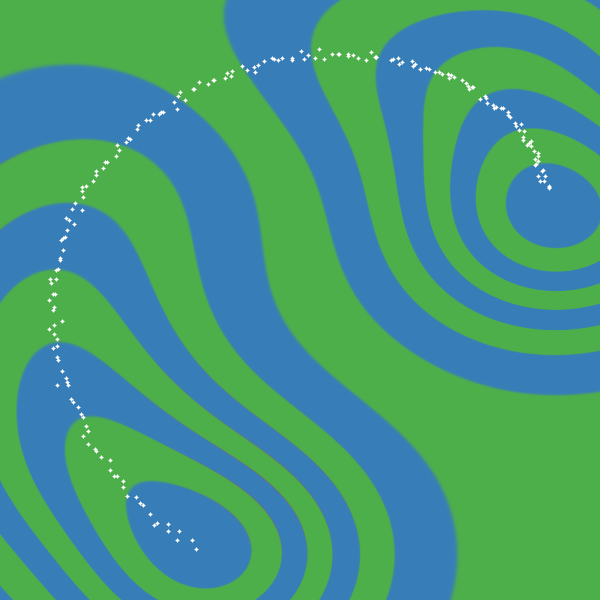
\includegraphics[clip, trim = 0cm 12cm 0cm 0.0cm, width=0.8\columnwidth]{figures/hidden_good}
    };
    \coordinate (D) at (1.6,1.5);
    \coordinate (Do) at (2.5, 0.8);
    \coordinate (Dt) at (3,3);
    
    \draw[pile] (D) -- (Dt) node[above, text width=5em] { tangent };
    \draw[pile] (D) -- (Do) node[right, text width=5em] { orthogonal };
\end{tikzpicture}
\end{center}

\begin{itemize}
	\item {\color{mydarkblue} Rifai et.\ al. (2011)}: good representations of data manifolds are invariant in directions orthogonal to the data manifold.
	\item Conversely, a good representation changes in directions tangent to the data manifold, to preserve information.
\end{itemize}


}


\newsavebox\deepkernels
\begin{lrbox}{\deepkernels}
  \begin{minipage}{0.4\textwidth}
%	({\color{blue}Cho, 2012}) built kernels from multiple layers of feature mappings.
Now our model is:
    \begin{align*}
%\feat(\vx) & = \vh^{(1)}(\vx) = \sigma \left( \vb^{(1)} + \vW^{(1)}\vx \right) \\
%f(\vx) & = \vV^{(1)} \sigma \left( \vb^{(1)} + \vW^{(1)} \vh^{(1)}(\vx) \right)  = \vV^{(1)} \vh^{(1)}(\vx) \\
 %= \frac{1}{K}{\mathbf \netweights}\tra \feat(\vx) 
f(\vx) = & \frac{1}{K} \sum_{i=1}^K \netweights_i \onefeat_i^{(2)} \! \left( \feat^{(1)}(\vx) \! \right) \\
= & \bm{\netweights}\tra \feat^{(2)} \left( \feat^{(1)}(\vx) \! \right)
    \end{align*} 
	Instead of 
	$$k_1(\vx, \vx') = \feat^{(1)}(\vx) \tra \feat^{(1)}(\vx'),$$
	we have ``deep kernel'':
	\begin{align*}
	& k_2(\vx, \vx') \\ 
	 & \!\! = \left[ \feat^{(2)} \! \left( \feat^{(1)}(\vx) \! \right) \right] \tra \! \feat^{(2)} \! \left( \feat^{(1)}(\vx') \! \right)
	\end{align*}
  \end{minipage}
\end{lrbox}


\frame[plain]{
\frametitle{Deep nets, deep kernels}
\begin{tabular}{c|c}
\begin{minipage}{0.535\textwidth}
\begin{tikzpicture}[shorten >=1pt,->,draw=black!50, node distance=\layersep]
\hspace{-1.4cm}
    \tikzstyle{every pin edge}=[<-,shorten <=1pt]
    \tikzstyle{neuron}=[circle,fill=black!25,minimum size=17pt,inner sep=0pt]
    \tikzstyle{input neuron}=[neuron, fill=green!30];
    \tikzstyle{output neuron}=[neuron, fill=red!30];
    \tikzstyle{hidden neuron}=[neuron, fill=blue!30];
    \tikzstyle{annot} = [text width=4em, text centered]

    % Draw the input layer nodes
    \foreach \name / \y in {1,...,\numdims}
    % This is the same as writing \foreach \name / \y in {1/1,2/2,3/3,4/4}
        \node[input neuron, minimum size=\nodesize
        %, pin=left:Input \#\y
        ] (I-\name) at (0,-\nodesep*\y) {$x_\y$};

    % Draw the hidden layer nodes
    \foreach \name / \y in {1,...,\numhidden}
        \path[yshift=0.5cm]
            node[hidden neuron, minimum size=\nodesize] (H-\name) at (\layersep,-\nodesep*\y) {$\onefeat^{(1)}_\y$};

    % Draw the hidden layer nodes
    \foreach \name / \y in {1,...,\numhidden}
        \path[yshift=0.5cm]
            node[hidden neuron, minimum size=\nodesize] (H2-\name) at (2*\layersep,-\nodesep*\y) {$\onefeat^{(2)}_\y$};

    % Draw the output layer node
    \foreach \name / \y in {1,...,\numouts}
    	\node[output neuron, minimum size=\nodesize
    	%,pin={[pin edge={->}]right:Output }
    	] (O-\name) at (2.8*\layersep,-\nodesep*2) {$f(\vx)$};

    % Connect every node in the input layer with every node in the
    % hidden layer.
    \foreach \source in {1,...,\numdims}
        \foreach \dest in {1,...,\numhidden}
            \path (I-\source) edge (H-\dest);
            
    \foreach \source in {1,...,\numhidden}
        \foreach \dest in {1,...,\numhidden}
            \path (H-\source) edge (H2-\dest);            

    % Connect every node in the hidden layer with the output layer
    \foreach \source in {1,...,\numhidden}
        \foreach \dest in {1,...,\numouts}
    	    \path (H2-\source) edge (O-\dest);

    % Annotate the layers
    \node[annot,above of=I-1, node distance=\upnodedist] {Inputs};
    \node[annot,above of=H-1, node distance=\upnodedist] {Hidden};
    \node[annot,above of=H2-1, node distance=\upnodedist] {Hidden};
    \node[annot,above of=O-1, node distance=\upnodedist] {Output};
\end{tikzpicture}
\end{minipage}
&
\usebox{\deepkernels}
  \end{tabular}
}



\newsavebox\deepkernelstwo
\begin{lrbox}{\deepkernelstwo}
  \begin{minipage}{0.4\textwidth}
%	({\color{blue}Cho, 2012}) built kernels from multiple layers of feature mappings.
Now our model is:
    \begin{align*}
\feat^{1}(x) = \left[ \sin(x), \cos(x) \right]
    \end{align*} 
	we have ``deep kernel'':
	\begin{align*}
	& k_2(\vx, \vx') \\ 
	& = \exp(-\frac{1}{2} \left( \feat^{1}(\vx)) - \feat^{1}(\vx') \right)
	\end{align*}
  \end{minipage}
\end{lrbox}

\newcommand{\numhiddenper}[0]{2}

\frame[plain]{
\frametitle{Example deep kernel: Periodic}
\begin{tabular}{c|c}
\begin{minipage}{0.535\textwidth}
\begin{tikzpicture}[shorten >=1pt,->,draw=black!50, node distance=\layersep]
\hspace{-1.4cm}
    \tikzstyle{every pin edge}=[<-,shorten <=1pt]
    \tikzstyle{neuron}=[circle,fill=black!25,minimum size=17pt,inner sep=0pt]
    \tikzstyle{input neuron}=[neuron, fill=green!30];
    \tikzstyle{output neuron}=[neuron, fill=red!30];
    \tikzstyle{hidden neuron}=[neuron, fill=blue!30];
    \tikzstyle{annot} = [text width=4em, text centered]

    % Draw the input layer nodes
    \foreach \name / \y in {1,...,1}
    % This is the same as writing \foreach \name / \y in {1/1,2/2,3/3,4/4}
        \node[input neuron, minimum size=\nodesize
        %, pin=left:Input \#\y
        ] (I-\name) at (0,-\nodesep*2) {$x$};

    % Draw the hidden layer nodes
%    \foreach \name / \y in {1,...,\numhiddenper}
    \path[yshift=0.5cm]
    node[hidden neuron, minimum size=\nodesize] (H-1) at (\layersep,-\nodesep*2) {$\sin(x)$};
   \path[yshift=0.5cm]
    node[hidden neuron, minimum size=\nodesize] (H-2) at (\layersep,-\nodesep*3) {$\cos(x)$};    

    % Draw the hidden layer nodes
    \foreach \name / \y in {1,...,\numhidden}
        \path[yshift=0.5cm]
            node[hidden neuron, minimum size=\nodesize] (H2-\name) at (2*\layersep,-\nodesep*\y) {$\onefeat^{(2)}_\y$};

    % Draw the output layer node
    \foreach \name / \y in {1,...,\numouts}
    	\node[output neuron, minimum size=\nodesize
    	%,pin={[pin edge={->}]right:Output }
    	] (O-\name) at (2.8*\layersep,-\nodesep*2) {$f(\vx)$};

    % Connect every node in the input layer with every node in the
    % hidden layer.
    \foreach \source in {1,...,1}
        \foreach \dest in {1,...,\numhiddenper}
            \path (I-\source) edge (H-\dest);
            
    \foreach \source in {1,...,\numhiddenper}
        \foreach \dest in {1,...,\numhidden}
            \path (H-\source) edge (H2-\dest);            

    % Connect every node in the hidden layer with the output layer
    \foreach \source in {1,...,\numhidden}
        \foreach \dest in {1,...,\numouts}
    	    \path (H2-\source) edge (O-\dest);

    % Annotate the layers
    \node[annot,above of=I-1, node distance=\upnodedist] {Inputs};
    \node[annot,above of=H-1, node distance=\upnodedist] {Hidden};
    \node[annot,above of=H2-1, node distance=\upnodedist] {Hidden};
    \node[annot,above of=O-1, node distance=\upnodedist] {Output};
\end{tikzpicture}
\end{minipage}
&
\usebox{\deepkernelstwo}
  \end{tabular}
}





\frame[plain]{
\frametitle{Deep Kernels}
\begin{itemize}
	\item ({\color{blue}Cho, 2012}) built kernels by composing feature mappings.
	\item Composing any kernel $k_1$ with a squared-exp kernel (SE):
%
\begin{align*}
%k_1(\vx, \vx') & = \exp \left( -\frac{1}{2} ||\vx - \vx'||_2^2 \right) \\
& k_2(\vx, \vx') = \\
& = \left( \feat^{SE} \left(\feat^{1}(\vx) \right) \right) \tra \feat^{SE} \left( \feat^{1}(\vx') \right) \\
& = \exp \left( -\frac{1}{2} || \feat^{1}(\vx) - \feat^{1}(\vx')||_2^2 \right) \nonumber\\
%k_{n+1}(\vx, \vx') 
%& = \exp \left( -\frac{1}{2} \sum_i \left[ \onefeat_n^{(i)}(\vx) - \onefeat_n^{(i)}(\vx') \right]^2 \right) \\
& = \exp\left ( -\frac{1}{2} \left[ \feat^{1}(\vx) \tra \feat^{1}(\vx) - 2 \feat^{1}(\vx) \tra \feat^{1}(\vx') + \feat^{1}(\vx') \tra \feat^{1}(\vx') \right] \right) \\
%k_2(\vx, \vx') & = \exp \left( -\frac{1}{2} \left[ \sum_i \onefeat_i(\vx)^2 - 2 \sum_i \onefeat_i(\vx) \onefeat_i(\vx') + \sum_i \onefeat_i(\vx')^2 \right] \right) \\
%k_{n+1}(\vx, \vx') 
& = \exp \left( -\frac{1}{2} \left[ k_1(\vx, \vx) - 2 k_1(\vx, \vx') + k_1(\vx', \vx') \right] \right)
%k_{n+1}(\vx, \vx') 
%& = \exp \left( k_1(\vx, \vx') - 1 \right) \qquad \textnormal{(if $k_1(\vx, \vx) = 1$)} \nonumber
\end{align*}
%
\item A closed form\dots let's do it again!
\end{itemize}
}




%\frame[plain]{
%\frametitle{Deep Kernels}
%
\includegraphics[height=0.4\textwidth]{figures/inception}
%}


\frame[plain]{
\frametitle{We need to go deeper}
%\begin{tabular}{c|c}
%\begin{minipage}{0.535\textwidth}
\begin{tikzpicture}[shorten >=1pt,->,draw=black!50, node distance=\layersep]
%\hspace{-1.4cm}
    \tikzstyle{every pin edge}=[<-,shorten <=1pt]
    \tikzstyle{neuron}=[circle,fill=black!25,minimum size=17pt,inner sep=0pt]
    \tikzstyle{input neuron}=[neuron, fill=green!30];
    \tikzstyle{output neuron}=[neuron, fill=red!30];
    \tikzstyle{hidden neuron}=[neuron, fill=blue!30];
    \tikzstyle{annot} = [text width=4em, text centered]

    % Draw the input layer nodes
    \foreach \name / \y in {1,...,\numdims}
    % This is the same as writing \foreach \name / \y in {1/1,2/2,3/3,4/4}
        \node[input neuron, minimum size=\nodesize
        %, pin=left:Input \#\y
        ] (I-\name) at (0,-\nodesep*\y) {$x_\y$};

    % Draw the hidden layer nodes
    \foreach \name / \y in {1,...,\numhidden}
        \path[yshift=0.5cm]
            node[hidden neuron, minimum size=\nodesize] (H-\name) at (\layersep,-\nodesep*\y) {$\onefeat^{(1)}_\y$};

    % Draw the hidden layer nodes
    \foreach \name / \y in {1,...,\numhidden}
        \path[yshift=0.5cm]
            node[hidden neuron, minimum size=\nodesize] (H2-\name) at (2*\layersep,-\nodesep*\y) {$\onefeat^{(2)}_\y$};
            
    % Draw the hidden layer nodes
    \foreach \name / \y in {1,...,\numhidden}
        \path[yshift=0.5cm]
            node[hidden neuron, minimum size=\nodesize] (H3-\name) at (3*\layersep,-\nodesep*\y) {$\onefeat^{(3)}_\y$};       
            
    % Draw the hidden layer nodes
    \foreach \name / \y in {1,...,\numhidden}
        \path[yshift=0.5cm]
            node[hidden neuron, minimum size=\nodesize] (H4-\name) at (4*\layersep,-\nodesep*\y) {$\onefeat^{(4)}_\y$};                    

    % Draw the output layer node
    \foreach \name / \y in {1,...,\numouts}
    	\node[output neuron, minimum size=\nodesize
    	%,pin={[pin edge={->}]right:Output }
    	] (O-\name) at (5*\layersep,-\nodesep*2) {$f(\vx)$};

    % Connect every node in the input layer with every node in the
    % hidden layer.
    \foreach \source in {1,...,\numdims}
        \foreach \dest in {1,...,\numhidden}
            \path (I-\source) edge (H-\dest);
            
    \foreach \source in {1,...,\numhidden}
        \foreach \dest in {1,...,\numhidden}
            \path (H-\source) edge (H2-\dest);  
            
    \foreach \source in {1,...,\numhidden}
        \foreach \dest in {1,...,\numhidden}
            \path (H2-\source) edge (H3-\dest);  
            
    \foreach \source in {1,...,\numhidden}
        \foreach \dest in {1,...,\numhidden}
            \path (H3-\source) edge (H4-\dest);                                    

    % Connect every node in the hidden layer with the output layer
    \foreach \source in {1,...,\numhidden}
        \foreach \dest in {1,...,\numouts}
    	    \path (H4-\source) edge (O-\dest);

    % Annotate the layers
%    \node[annot,above of=I-1, node distance=\upnodedist] {Inputs};
%    \node[annot,above of=H-1, node distance=\upnodedist] {Hidden};
%    \node[annot,above of=H2-1, node distance=\upnodedist] {Hidden};
%    \node[annot,above of=O-1, node distance=\upnodedist] {Output};
\end{tikzpicture}
%\end{minipage}
%&
%\usebox{\deepkernels}
%  \end{tabular}
}





\frame[plain]{
\frametitle{Infinitely Deep Kernels}
\begin{itemize}
	\item For SE kernel, $k_{L+1}(\vx, \vx') = \exp \left( k_L(\vx, \vx') - 1 \right)$.
	\item What is the limit of composing SE features?
\end{itemize}
\centering
\begin{tabular}{cc}
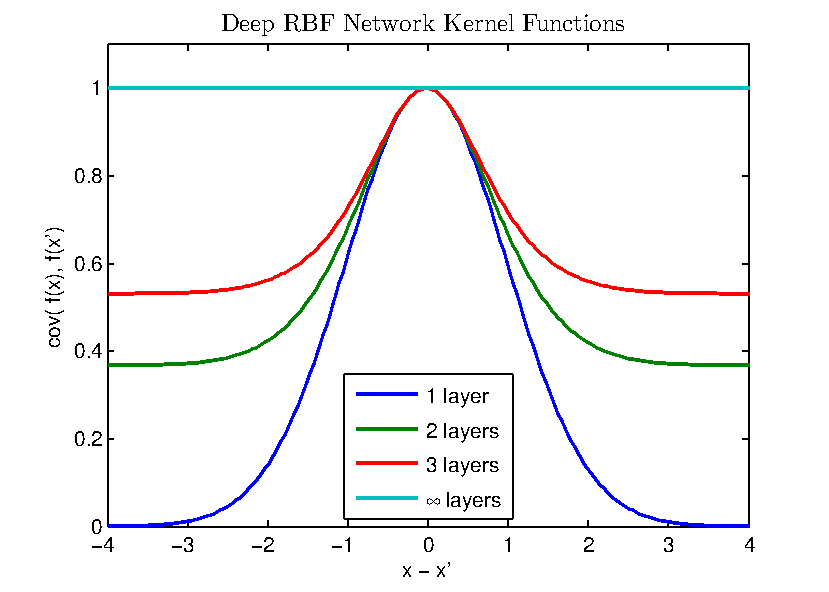
\includegraphics[width=0.55\columnwidth, clip, trim = 0cm 0cm 0cm 0.61cm]{figures/deep_kernel} &
\hspace{-1cm}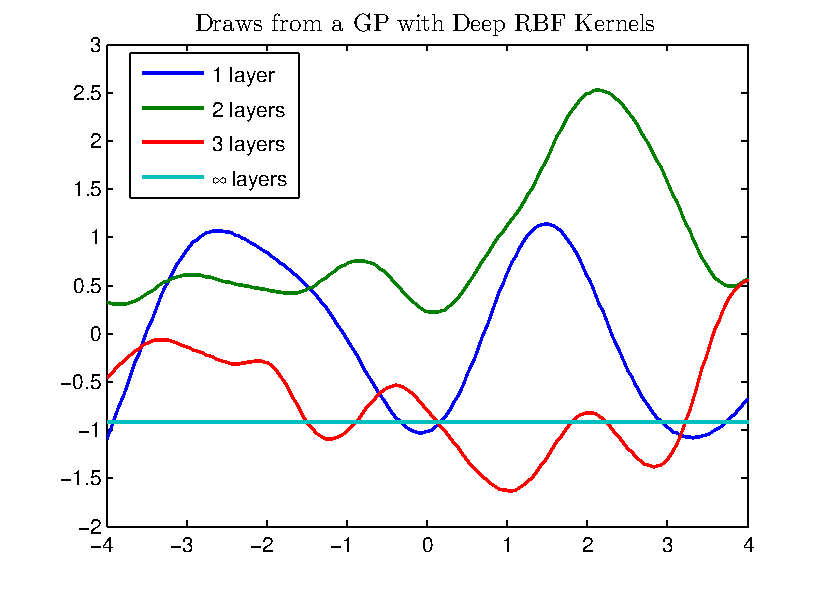
\includegraphics[width=0.55\columnwidth, clip, trim = 0cm 0cm 0cm 0.61cm]{figures/deep_kernel_draws} \\
Kernel & Draws from GP prior
\end{tabular}

\begin{itemize}
	\item $k_\infty(\vx, \vx') = 1$ everywhere.  \frownie
\end{itemize}
}



\frame[plain]{
\frametitle{A simple fix...}
\begin{itemize}
	\item Following a suggestion from {\color{blue!80} Neal (1995)}, we 
connect the inputs $\vx$ to each layer:

\vspace{0.5cm}

%\def\layersep{1.33cm}
\def\nodeseptwo{1.8cm}
%\def\nodesize{.35cm}

%\newcommand{\numdims}[0]{3}
%\newcommand{\numhidden}[0]{4}
%\newcommand{\upnodedist}[0]{0.6cm}
%\newcommand{\bardist}[0]{\hspace{-0.2cm}}

\begin{tabular}{c}
\bardist
Standard architecture: \\
\begin{tikzpicture}[draw=black!80]
    \tikzstyle{neuron}=[circle,minimum size=17pt, draw = black!80, fill = white, thick]
    \tikzstyle{input neuron}=[neuron, fill=green!50];
    \tikzstyle{output neuron}=[neuron, fill=red!50];
    \tikzstyle{hidden neuron}=[neuron, fill=blue!50];
    \tikzstyle{pile} =[thick, ->, >=stealth', shorten <=7pt, shorten >=8pt];

    % Define the input layer node
    \coordinate (I) at (0, 0);


    % Define the hidden layer nodes
    \foreach \name / \i in {1,...,\numhidden}
    {
        \coordinate (H-\name) at (\nodeseptwo * \i, 0);
    }

    % Connect every node            
    \foreach \name in {1,...,\numhidden}
    {
	 \path[pile] (I) edge (H-\name) {};
         %\path[pile] (I) edge [bend left] (H-\name) {};
    }

    \draw (I) node[neuron] {};
    \draw (I) node[below = 0.5cm]  {$\vx$};

    % Draw the hidden layer nodes
    \foreach \name / \y in {1,...,\numhidden}
    {
	\draw (H-\name) node[neuron]  {};
        \draw (H-\name) node[below = 0.34cm] {$\vf^{(\y)}(\vx)$};
    }
\end{tikzpicture} \\
\vspace{\baselineskip}
\\
Input-connected architecture: \\
\bardist
\begin{tikzpicture}[draw=black!80]
    \tikzstyle{neuron}=[circle,minimum size=17pt, draw = black!80, fill = white, thick]
    \tikzstyle{input neuron}=[neuron, fill=green!50];
    \tikzstyle{output neuron}=[neuron, fill=red!50];
    \tikzstyle{hidden neuron}=[neuron, fill=blue!50];
    \tikzstyle{pile} =[thick, ->, >=stealth', shorten <=7pt, shorten >=8pt];

    % Define the input layer node
    \coordinate (I) at (0, 0);


    % Define the hidden layer nodes
    \foreach \name / \y in {1,...,\numhidden}
    {
        \coordinate (H-\name) at (\nodeseptwo*\y, 0);
    }

    % Connect every node            
    \path[pile] (I) edge (H-1) {};
    \foreach \name in {2,...,\numhidden}
    {
	 \path[pile] (I) edge (H-\name) {};
         \path[pile] (I) edge [bend left] (H-\name) {};
    }

    \draw (I) node[neuron] {};
    \draw (I) node[below = 0.5cm]  {$\vx$};

    % Draw the hidden layer nodes
    \foreach \name / \y in {1,...,\numhidden}
    {
	\draw (H-\name) node[neuron]  {};
        \draw (H-\name) node[below = 0.34cm] {$\vf^{(\y)}(\vx)$};
    }
\end{tikzpicture} 
\end{tabular}

\end{itemize}
}



\frame[plain]{
\frametitle{A simple fix...}
\begin{itemize}
	\item Following a suggestion from {\color{blue!80} Neal (1995)}, we 
connect the inputs $\vx$ to each layer:
%
\begin{align*}
%k_1(\vx, \vx') & = \exp \left( -\frac{1}{2} ||\vx - \vx'||_2^2 \right) \\
& k_{L+1}(\vx, \vx') = \nonumber \\
& = \exp \left( -\frac{1}{2} \left|\left| \left[ \! \begin{array}{c} \feat^L(\vx) \\ {\color{red} \vx} \end{array} \! \right]  - \left[ \! \begin{array}{c} \feat^L(\vx') \\ {\color{red} \vx'} \end{array} \! \right] \right| \right|_2^2 \right) \nonumber \\
%k_{n+1}(\vx, \vx') 
%& = \exp \left( -\frac{1}{2} \sum_i \left[ \onefeat_i(\vx) - \onefeat_i(\vx') \right]^2 -\frac{1}{2} || \vx - \vx' ||_2^2 \right) \\
%k_{n+1}(\vx, \vx') & = \exp\left ( -\frac{1}{2} \sum_i \left[ \onefeat_i(\vx)^2 - 2 \onefeat_i(\vx) \onefeat_i(\vx') + \onefeat_i(\vx')^2 \right]  -\frac{1}{2} || \vx - \vx' ||_2^2 \right) \\
%k_2(\vx, \vx') & = \exp \left( -\frac{1}{2} \left[ \sum_i \onefeat_i(\vx)^2 - 2 \sum_i \onefeat_i(\vx) \onefeat_i(\vx') + \sum_i \onefeat_i(\vx')^2 \right] \right) \\
%k_2(\vx, \vx') & = \exp \left( -\frac{1}{2} \left[ k_1(\vx, \vx) - 2 k_1(\vx, \vx') + k_1(\vx', \vx') \right] \right) \\
%k_{n+1}(\vx, \vx') 
& = \exp \left( -\frac{1}{2} \left[ k_L(\vx, \vx) - 2 k_L(\vx, \vx') + k_L(\vx', \vx') \right] {\color{red} -\frac{1}{2} || \vx - \vx' ||_2^2} \right)
\end{align*}
%\item What is the eventual limit?
\end{itemize}
}


\frame[plain]{
\frametitle{Infinitely Deep Kernels}
\begin{itemize}
	\item What is the limit of compositions of input-connected SE features?
	\item $k_{L+1}(\vx, \vx') = \exp \left( k_L(\vx, \vx') - 1 -\frac{1}{2} || \vx - \vx' ||_2^2 \right)$.	
\end{itemize}
\centering
\begin{tabular}{cc}
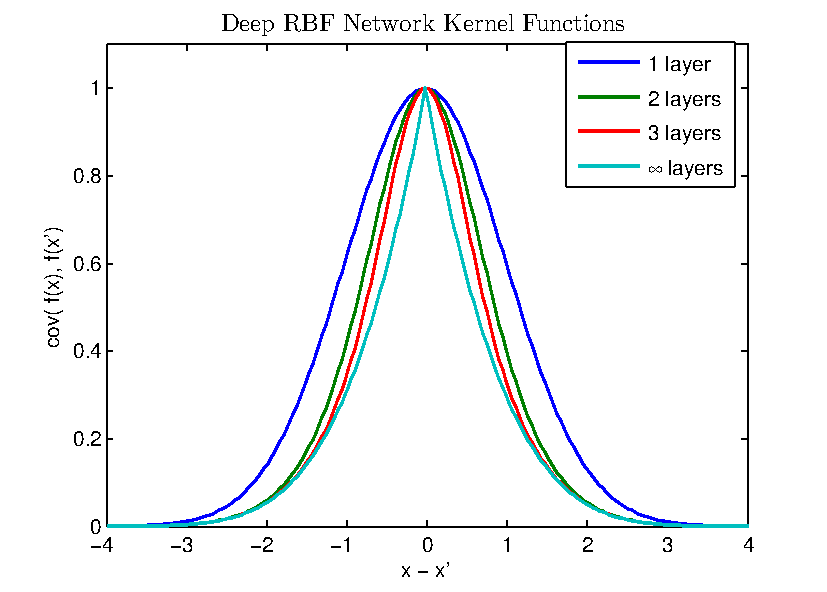
\includegraphics[width=0.56\columnwidth, clip, trim = 0cm 0cm 0cm 0.61cm]{figures/deep_kernel_connected} &
\hspace{-1cm}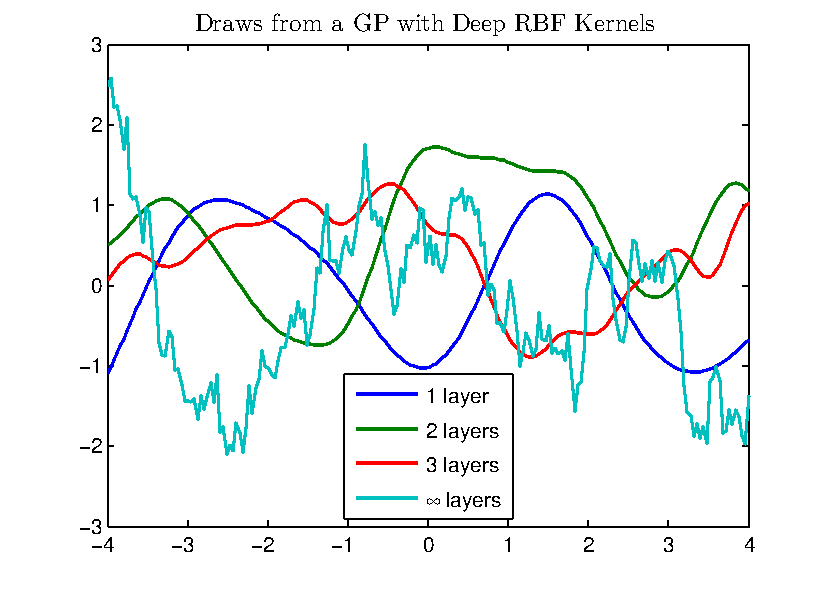
\includegraphics[width=0.55\columnwidth, clip, trim = 0cm 0cm 0cm 0.61cm]{figures/deep_kernel_connected_draws} \\
Kernels & Draws from GP priors
\end{tabular}

\begin{itemize}
	\item Like an Ornstein-Uhlenbeck process with skinny tails
	\item Samples are non-differentiable (fractal).
\end{itemize}
}


\frame[plain]{
\frametitle{What went wrong?}
\begin{itemize}
	\item Fixed feature mapping, unlikely to be useful for anything
%	\item only one type of structure repeated
%	\item not capturing invariances?
%	\item not throwing away unnecessary information
	\item power of neural nets comes from learning a custom representation
	\item Need to search over feature mappings!
	\item Can try to learn kernels, or even better, integrate over feature mappings
\end{itemize}
}





%\newcommand{\numdims}[0]{3}
%\newcommand{\numouts}[0]{1}
%\newcommand{\numhidden}[0]{4}
%\newcommand{\upnodedist}[0]{1cm}
%\newcommand{\bardist}[0]{\hspace{-0.2cm}}

\frame[plain]{
\frametitle{Deep Gaussian Processes}
\begin{tikzpicture}[shorten >=1pt,->,draw=black!50, node distance=\layersep]
    \tikzstyle{every pin edge}=[<-,shorten <=1pt]
    \tikzstyle{neuron}=[circle,fill=black!25,minimum size=17pt,inner sep=0pt]
    \tikzstyle{input neuron}=[neuron, fill=green!50];
    \tikzstyle{output neuron}=[neuron, fill=red!50];
    \tikzstyle{hidden neuron}=[neuron, fill=blue!50];
    \tikzstyle{annot} = [text width=4em, text centered]

    % Draw the input layer nodes
    \foreach \name / \y in {1,...,\numdims}
    % This is the same as writing \foreach \name / \y in {1/1,2/2,3/3,4/4}
        \node[input neuron, minimum size=\nodesize
        %, pin=left:Input \#\y
        ] (I-\name) at (0,-\nodesep*\y) {$x_\y$};

    % Draw the hidden layer nodes
    \foreach \name / \y in {1,...,\numhidden}
        \path[yshift=0.5cm]
            node[hidden neuron, minimum size=\nodesize] (H-\name) at (\layersep,-\nodesep*\y)  {$\onefeat^{(1)}_\y$};

    % Draw the hidden layer nodes
    \foreach \name / \y in {1,...,\numhidden}
        \path[yshift=0.5cm]
            node[hidden neuron, minimum size=\nodesize] (H2-\name) at (3*\layersep,-\nodesep*\y)  {$\onefeat^{(2)}_\y$};

    % Draw the output layer node
    \foreach \name / \y in {1,...,\numdims}
    	\node[output neuron, minimum size=\nodesize
    	%,pin={[pin edge={->}]right:Output }
    	] (O1-\name) at (2*\layersep,-\nodesep*\y) {$f^{(1)}_\y$};

    % Draw the output layer node
    \foreach \name / \y in {1,...,\numdims}
    	\node[output neuron, minimum size=\nodesize
    	%,pin={[pin edge={->}]right:Output }
    	] (O2-\name) at (4*\layersep,-\nodesep*\y) {$f^{(1:2)}_\y$};

    % Connect every node in the input layer with every node in the
    % hidden layer.
    \foreach \source in {1,...,\numdims}
        \foreach \dest in {1,...,\numhidden}
            \path (I-\source) edge (H-\dest);
            
    \foreach \source in {1,...,\numhidden}
        \foreach \dest in {1,...,\numdims}
            \path (H-\source) edge (O1-\dest);         
            
    \foreach \source in {1,...,\numdims}
        \foreach \dest in {1,...,\numhidden}
            \path (O1-\source) edge (H2-\dest);                

    % Connect every node in the hidden layer with the output layer
    \foreach \source in {1,...,\numhidden}
        \foreach \dest in {1,...,\numdims}
    	    \path (H2-\source) edge (O2-\dest);

    % Annotate the layers
    \node[annot,above of=I-1, node distance=\upnodedist] {Inputs};
    \node[annot,above of=H-1, node distance=\upnodedist] {Hidden};
    \node[annot,above of=O1-1, node distance=\upnodedist] {$\vf^{(1)}(\vx)$};
    \node[annot,above of=H2-1, node distance=\upnodedist] {Hidden};
    \node[annot,above of=O2-1, node distance=\upnodedist] {$\vf^{(1:2)}(\vx)$};

\end{tikzpicture}
}


\def\ie{i.e.\ }
\def\eg{e.g.\ }
\def\iid{i.i.d.\ }
%\def\simiid{\sim_{\mbox{\tiny iid}}}
\def\simiid{\overset{\mbox{\tiny iid}}{\sim}}
\def\simind{\overset{\mbox{\tiny \textnormal{ind}}}{\sim}}
\def\eqdist{\stackrel{\mbox{\tiny d}}{=}}
\newcommand{\distas}[1]{\mathbin{\overset{#1}{\kern\z@\sim}}}
%\newcommand{\vf}{\vect{f}}
\newcommand{\GPt}[2]{\mathcal{GP}\!\left(#1,#2\right)}

\frame[plain]{
\frametitle{Deep Gaussian Processes}
\begin{itemize}
	\item a prior over compositions of functions:
	\begin{align}
\vf^{(1:L)}(\vx) = \vf^{(L)}(\vf^{(L-1)}(\dots \vf^{(2)}(\vf^{(1)}(\vx)) \dots))
\end{align}
%
where each $\vf_d^{(\ell)} \simind \GPt{0}{k^\ell_d(\vx, \vx')}$. 
	\item Analogous to neural nets, where each neuron's activation function is an independent draw from a GP.
	\item inference is really hard.	
	\item maybe we can learn something just from looking at draws?
\end{itemize}
}

\newcommand{\onedsamplepic}[1]{
\includegraphics[width=0.7\columnwidth]{figures/1d_samples/latent_seed_0_1d_large/layer-#1}}

\frame[plain]{
\frametitle{Deep Gaussian Processes}
\begin{itemize}
	\item Draws from one-dimensional deep GPs:
	\vspace{\baselineskip}
	\only<1>{\onedsamplepic{1}}
	\only<2>{\onedsamplepic{2}}
	\only<3>{\onedsamplepic{3}}
	\only<4>{\onedsamplepic{4}}
	\only<5>{\onedsamplepic{5}}
	\only<6>{\onedsamplepic{6}}
	\only<7>{\onedsamplepic{7}}
	\only<8>{\onedsamplepic{8}}
	\only<9>{\onedsamplepic{9}}
	\only<10>{\onedsamplepic{10}}
\end{itemize}
}


\newcommand{\gpdrawbox}[1]{
\setlength\fboxsep{0pt}
\fbox{
\includegraphics[width=0.67\columnwidth]{figures/deep_draws/deep_gp_sample_layer_#1}
}}

\frame[plain]{
\frametitle{Deep Gaussian Processes}
\begin{itemize}
	\item 2D to 2D warpings of a Gaussian density:
	\vspace{\baselineskip}
	\only<1>{\gpdrawbox{1}}
	\only<2>{\gpdrawbox{2}}
	\only<3>{\gpdrawbox{3}}
	\only<4>{\gpdrawbox{4}}
	\only<5>{\gpdrawbox{5}}
	\only<6>{\gpdrawbox{6}}
\end{itemize}
}





\newcommand{\mappic}[1]{
%\includegraphics[width=0.6\columnwidth]{figures/map/latent_coord_map_layer_#1}
\includegraphics[width=0.67\columnwidth]{figures/seed-0-map/latent_coord_map_layer_#1}
} 
\newcommand{\mappiccon}[1]{
\includegraphics[width=0.67\columnwidth]{figures/seed-0-map-connected/latent_coord_map_layer_#1}
%\includegraphics[width=0.6\columnwidth]{figures/map_connected/latent_coord_map_layer_#1}
}


\frame[plain]{
\frametitle{Deep Gaussian Processes}
\begin{itemize}
	\item Showing the x that gave rise to a particular y
	\item (i.e. decision boundaries) \\
	\vspace{\baselineskip}
	\only<1>{\mappic{0} \quad No warping}
	\only<2>{\mappic{1} \quad One Layers}
	\only<3>{\mappic{2} \quad Two Layers}
	\only<4>{\mappic{3} \quad Three Layers}
	\only<5>{\mappic{4} \quad Four Layers}
	\only<6>{\mappic{5} \quad Five Layers}
	\only<7>{\mappic{10} \quad Ten Layers}
	\only<8>{\mappic{20} \quad Twenty Layers}
	\only<9>{\mappic{40} \quad Forty Layers}
\end{itemize}
}

\frame[plain]{
\frametitle{Deep Gaussian Processes}
\begin{itemize}
	\item Only one degree of freedom in $x$ is being captured!
	\item Again following Radford's thesis, connect every layer to input:
	 %\def\layersep{1.33cm}
\def\nodeseptwo{1.8cm}
%\def\nodesize{.35cm}

%\newcommand{\numdims}[0]{3}
%\newcommand{\numhidden}[0]{4}
%\newcommand{\upnodedist}[0]{0.6cm}
%\newcommand{\bardist}[0]{\hspace{-0.2cm}}

\begin{tabular}{c}
\bardist
Standard architecture: \\
\begin{tikzpicture}[draw=black!80]
    \tikzstyle{neuron}=[circle,minimum size=17pt, draw = black!80, fill = white, thick]
    \tikzstyle{input neuron}=[neuron, fill=green!50];
    \tikzstyle{output neuron}=[neuron, fill=red!50];
    \tikzstyle{hidden neuron}=[neuron, fill=blue!50];
    \tikzstyle{pile} =[thick, ->, >=stealth', shorten <=7pt, shorten >=8pt];

    % Define the input layer node
    \coordinate (I) at (0, 0);


    % Define the hidden layer nodes
    \foreach \name / \i in {1,...,\numhidden}
    {
        \coordinate (H-\name) at (\nodeseptwo * \i, 0);
    }

    % Connect every node            
    \foreach \name in {1,...,\numhidden}
    {
	 \path[pile] (I) edge (H-\name) {};
         %\path[pile] (I) edge [bend left] (H-\name) {};
    }

    \draw (I) node[neuron] {};
    \draw (I) node[below = 0.5cm]  {$\vx$};

    % Draw the hidden layer nodes
    \foreach \name / \y in {1,...,\numhidden}
    {
	\draw (H-\name) node[neuron]  {};
        \draw (H-\name) node[below = 0.34cm] {$\vf^{(\y)}(\vx)$};
    }
\end{tikzpicture} \\
\vspace{\baselineskip}
\\
Input-connected architecture: \\
\bardist
\begin{tikzpicture}[draw=black!80]
    \tikzstyle{neuron}=[circle,minimum size=17pt, draw = black!80, fill = white, thick]
    \tikzstyle{input neuron}=[neuron, fill=green!50];
    \tikzstyle{output neuron}=[neuron, fill=red!50];
    \tikzstyle{hidden neuron}=[neuron, fill=blue!50];
    \tikzstyle{pile} =[thick, ->, >=stealth', shorten <=7pt, shorten >=8pt];

    % Define the input layer node
    \coordinate (I) at (0, 0);


    % Define the hidden layer nodes
    \foreach \name / \y in {1,...,\numhidden}
    {
        \coordinate (H-\name) at (\nodeseptwo*\y, 0);
    }

    % Connect every node            
    \path[pile] (I) edge (H-1) {};
    \foreach \name in {2,...,\numhidden}
    {
	 \path[pile] (I) edge (H-\name) {};
         \path[pile] (I) edge [bend left] (H-\name) {};
    }

    \draw (I) node[neuron] {};
    \draw (I) node[below = 0.5cm]  {$\vx$};

    % Draw the hidden layer nodes
    \foreach \name / \y in {1,...,\numhidden}
    {
	\draw (H-\name) node[neuron]  {};
        \draw (H-\name) node[below = 0.34cm] {$\vf^{(\y)}(\vx)$};
    }
\end{tikzpicture} 
\end{tabular}

\end{itemize}
}


\newcommand{\onedsamplepiccon}[1]{
\includegraphics[width=0.7\columnwidth]{figures/1d_samples/latent_seed_0_1d_large_connected/layer-#1}
%\includegraphics[width=0.67\columnwidth]{figures/seed-0-map/latent_coord_map_layer_#1}%
}

\frame[plain]{
\frametitle{Deep Gaussian Processes}
\begin{itemize}
	\item Draws from input-connected one-dimensional deep GPs:
	\vspace{\baselineskip}
	\only<1>{\onedsamplepiccon{1}}
	\only<2>{\onedsamplepiccon{2}}
	\only<3>{\onedsamplepiccon{3}}
	\only<4>{\onedsamplepiccon{4}}
	\only<5>{\onedsamplepiccon{5}}
	\only<6>{\onedsamplepiccon{6}}
	\only<7>{\onedsamplepiccon{7}}
	\only<8>{\onedsamplepiccon{8}}
	\only<9>{\onedsamplepiccon{9}}
	\only<10>{\onedsamplepiccon{10}}
\end{itemize}
}


\newcommand{\gpdrawboxcon}[1]{
\setlength\fboxsep{0pt}
\fbox{
\includegraphics[width=0.67\columnwidth]{figures/deep_draws_connected/deep_sample_connected_layer#1}%
}}%

\frame[plain]{
\frametitle{Deep Gaussian Processes}
\begin{itemize}
	\item input-connected 2D to 2D warpings of a Gaussian density:
	\vspace{\baselineskip}
	\only<1>{\gpdrawbox{1}}%
	\only<2>{\gpdrawboxcon{2}}%
	\only<3>{\gpdrawboxcon{3}}%
	\only<4>{\gpdrawboxcon{4}}%
	\only<5>{\gpdrawboxcon{5}}%
	\only<6>{\gpdrawboxcon{6}}%
\end{itemize}
}




\frame[plain]{
\frametitle{Deep Gaussian Processes}
\begin{itemize}
	\item Showing the x that gave rise to a particular y
	\item (i.e. decision boundaries) \\
	\vspace{\baselineskip}
	\only<1>{\mappic{0} \quad No warping}
	\only<2>{\mappiccon{2} \quad Two Layers}
	\only<3>{\mappiccon{10} \quad Ten Layers}
	\only<4>{\mappiccon{20} \quad Twenty Layers}
	\only<5>{\mappiccon{40} \quad Forty Layers}
\end{itemize}
}



\frame[plain]{
\frametitle{Dropout}
\begin{itemize}
	\item Dropout is a method for regularizing neural networks {\color{mydarkblue} (Hinton et al.,
2012; Srivastava, 2013)}.
	\item Recipe:
	\begin{enumerate}
		\item randomly set half of feature activations to zero
		\item Double the remaining features activations
		\item Average over all possible ways of dropping out
	\end{enumerate}
	\item Gives robustness, since neurons can't depend on one another.
	\item What do we get when we do dropout in GPs?
\end{itemize}
}




\newcommand{\numhiddentwo}[0]{5}

\frame[plain]{
\frametitle{Dropout on Feature Activations}

%\vspace{0.5cm}
\begin{tabular}{c|c}
\hspace{-1cm}
\begin{minipage}{0.5\textwidth}
\begin{tikzpicture}[shorten >=1pt,->,draw=black!50, node distance=\layersep]
    \tikzstyle{every pin edge}=[<-,shorten <=1pt]
    \tikzstyle{neuron}=[circle,fill=black!25,minimum size=17pt,inner sep=0pt]
    \tikzstyle{input neuron}=[neuron, fill=green!30];
    \tikzstyle{output neuron}=[neuron, fill=red!30];
    \tikzstyle{hidden neuron}=[neuron, fill=blue!30];
    \tikzstyle{annot} = [text width=4em, text centered]

    % Draw the input layer nodes
    \foreach \name / \y in {1,...,\numdims}
    % This is the same as writing \foreach \name / \y in {1/1,2/2,3/3,4/4}
        \node[input neuron, minimum size=\nodesize
        %, pin=left:Input \#\y
        ] (I-\name) at (0,-\nodesep*\y) {$x_\y$};

    % Draw the hidden layer nodes
    \foreach \name / \y in {1,...,\numhiddentwo}
        \path[yshift=1.5cm]
            node[hidden neuron, minimum size=\nodesize] (H-\name) at (\layersep,-\nodesep*\y) {$\onefeat_\y(\vx)$};

    % Draw the output layer node
    \foreach \name / \y in {1,...,\numouts}
    	\node[output neuron, minimum size=\nodesize
    	%,pin={[pin edge={->}]right:Output }
    	] (O-\name) at (2*\layersep,-\nodesep*2) {$f(x)$};

    % Connect every node in the input layer with every node in the
    % hidden layer.
    \foreach \source in {1,...,\numdims}
        \foreach \dest in {1,...,\numhiddentwo}
            \path (I-\source) edge (H-\dest);

    % Connect every node in the hidden layer with the output layer
%    \foreach \source in {1,...,\numhiddentwo}
 %       \foreach \dest in {1,...,\numouts}
    \only<1,2,3,5,7,9> {\path (H-1) [thick] edge (O-1);}
    \only<1,3,4,6,8,10> {\path (H-2) [thick] edge (O-1);}
    \only<1,3,2,3,6,7,10> {\path (H-3) [thick] edge (O-1);}
    \only<1,2,2,4,5,8,9> {\path (H-4) [thick] edge (O-1);}
    \only<1,2,2,3,6,8,10> {\path (H-5) [thick] edge (O-1);}

    \only<11>{\path (H-2) [black,thick] edge (O-1);}
    \only<11>{\path (H-3) [black,thick] edge (O-1);}
    \only<11>{\path (H-5) [black,thick] edge (O-1);}

    % Annotate the layers
%    \node[annot,above of=I-1, node distance=\upnodedist] {Inputs};
%    \node[annot,above of=H-1, node distance=\upnodedist] {Hidden};
%    \node[annot,above of=O-1, node distance=\upnodedist] {Output};
\end{tikzpicture} 
\end{minipage}
&
\begin{minipage}{0.53\textwidth}
\only<1>{Original formulation:}
\only<2-10>{Remove units with probability \nicefrac{1}{2}:}
\only<11>{Double output variance:}

$$f(\vx) = \frac{\only<1-10>{1} \only<11>{{\color{green}2}}}{K} \sum_{i=1}^K \only<2-11>{{\color{red}r_i}} \netweights_i \onefeat_i(\vx) \quad \only<2-11>{{\color{red}r_i} \simiid \textnormal{Ber}(\nicefrac{1}{2})}$$
with any weight distribution,
$$\expectargs{}{\only<11>{{\color{green}2}}\only<2-11>{{\color{red}r_i}} \netweights_i} = 0, \quad \varianceargs{}{\only<11>{{\color{green}2}} \only<2-11>{{\color{red}r_i}} \netweights_i} = 
\only<2-10>{{\color{red}\frac{1}{4}}}
\only<11>{{\color{green}\frac{4}{4}}}\sigma^2$$
by CLT, gives a GP as $K \to \infty$
$$\cov \left[ \! \begin{array}{c} f(\vx) \\ f(\vx') \end{array} \! \right] \to 
\only<2-10>{{\color{red}\frac{1}{4}}}
\only<11>{{\color{green}\frac{4}{4}}}
\frac{\sigma^2}{K}\sum_{i=1}^K \onefeat_i(\vx)\onefeat_i(\vx')$$
\end{minipage}
  \end{tabular}
}




\frame[plain]{
\frametitle{Dropout on Feature Activations}
\begin{itemize}
	\item Dropout on feature activations gives same GP
	\begin{itemize}
	\item Averaging the same model doesn't do anything
	 \end{itemize}
	\item GPs were doing dropout all along?	\smiley
	\item GPs strange because any one feature doesn't matter.
	\item Is there a better way to drop out features that would lead to robustness?
\end{itemize}
}


\frame[plain]{
\frametitle{Dropout on Inputs}
\begin{itemize}
%	\item Let $\vx$ be $D$ dimensional.
	\item Let $k(\vx, \vx') = \prod_{d=1}^D k_d(\vx_d, \vx_d')$
	\item Exact averaging over all dropouts is a mixture of GPs:$$ p(f(\vx)))= \frac{1}{2^D} \sum_{\vr \in \{0,1\}^D}  \gp \left(0, \prod_{d=1}^D k_d(\vx_d, \vx_d')^{r_d} \right)$$
	\item Probably a nice model, but presumably intractable.
	\item In neural net literature, exponentially-many dropout models are averaged over in tractable ways.
	\item For instance, dropout mixture has same covariance as $$ f(\vx) \sim \gp \left(0, \frac{1}{2^D} \sum_{\vr \in \{0,1\}^D}  \prod_{d=1}^D k_d(\vx_d, \vx_d')^{r_d} \right)$$
\end{itemize}
}


\frame[plain]{
\frametitle{Dropout on Inputs}
$$ f(\vx) \sim \gp \left(0, \sum_{\vr \in \{0,1\}^D}  \prod_{d=1}^D k_d(\vx_d, \vx_d')^{r_d} \right)$$
\begin{itemize}
	\item That's exactly additive GPs!  Kernel isocontours look like:
	\hspace*{-8pt}\makebox[\linewidth][c]{
\centering
\begin{tabular}{cccc}
\hspace{-0.2in} 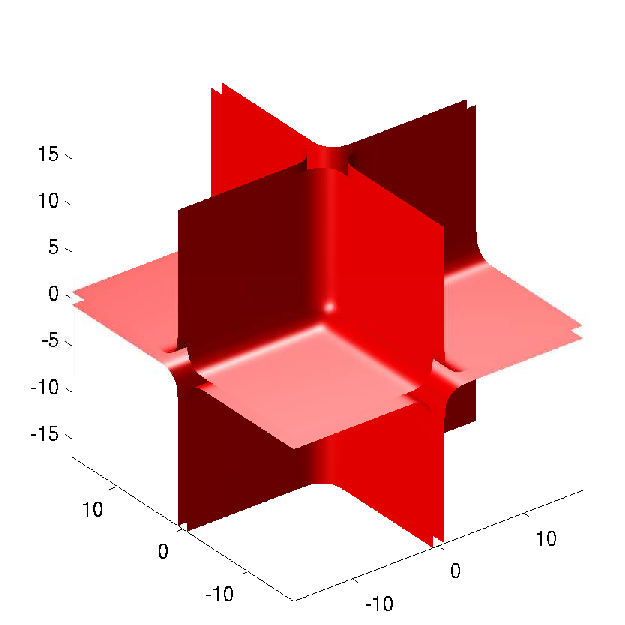
\includegraphics[width=0.27\textwidth]{figures/3d_add_kernel_1.pdf} &
\hspace{-0.2in} 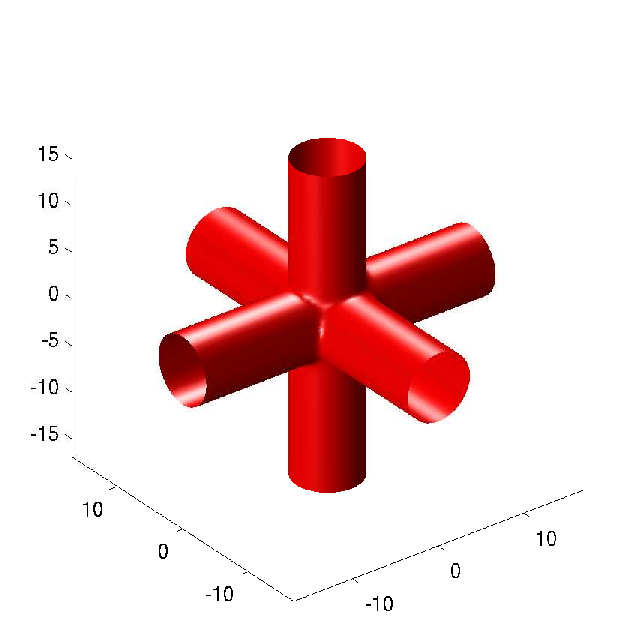
\includegraphics[width=0.27\textwidth]{figures/3d_add_kernel_2.pdf} &
\hspace{-0.2in} 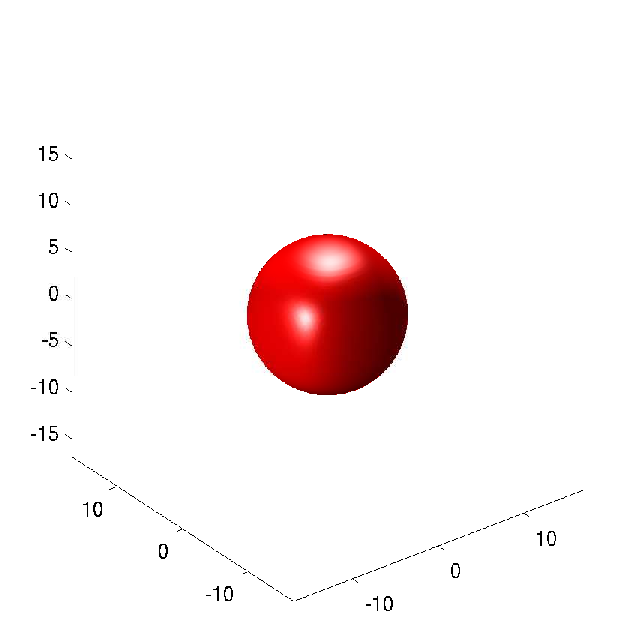
\includegraphics[width=0.27\textwidth]{figures/3d_add_kernel_3.pdf} & 
\hspace{-0.2in} 
\includegraphics[width=0.27\textwidth]{figures/3d_add_kernel_321.pdf}\\
%1st order interactions & 2nd order interactions & 3rd order interactions & All interactions \\
$k_1 + k_2 + k_3$ & $k_1k_2 + k_2k_3 + k_1k_3$ & $k_1k_2k_3$ & all terms\\
%& & (Squared-exp kernel) & (Additive kernel)\\
\end{tabular}
}
	\item Can compute all $2^D$ terms in $\mathcal{O}(D^2)$
	\item lots of functions, each only depends on some of the inputs
\end{itemize}
}



%\setbeamertemplate{background canvas}{\begin{tikzpicture}\node[opacity=.1]{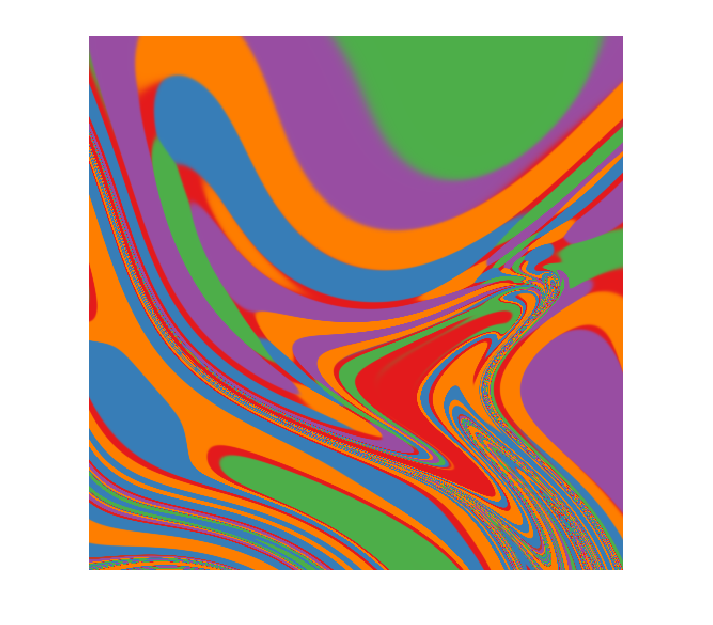
\includegraphics [width=\paperwidth]{figures/map_connected/latent_coord_map_layer_40}};\end{tikzpicture}}

\frame[plain]{
\frametitle{Summary}
\begin{itemize}
	\item At least two different ways to make GPs deep:
	\begin{itemize}
		\item composing kernels (inference easy, have to specify kernel)
		\item composing GPs (inference is hard, but can learn structure)
	\end{itemize}
%	\vspace{\baselineskip}
	\item Kernel learning is a form of representation learning
	\vspace{\baselineskip}
	\item Building priors over functions can shed light on architectures choices or initialization strategies in a data-independent way.
	\item What sorts of structures do we want to be able to learn? 
	\vspace{\baselineskip}
	\item We can bring tricks from the neural net literature back to GPs. (still need to try translation-invariant image kernels!)	
%	\item Open questions:
%	\begin{itemize}
%		\item When is discrete kernel search a good way to find representations?
%		\item What could we do if we could compute the marginal likelihood of a neural net?
%	\end{itemize}
\end{itemize}
	\pause
	\centering
	{
		\hfill
		{\color{blue} Thanks!}
				\hfill
	}
}


\end{document}

